% Created 2015-02-20 Пт 06:18
\documentclass[presentation]{beamer}
\useoutertheme[subsection=true]{miniframes}%{miniframes}

%%% Packages.

\usepackage[utf8]{inputenc}
\usepackage[T1]{fontenc}
\usepackage{fixltx2e}
\usepackage{graphicx}
\usepackage{longtable}
\usepackage{float}
\usepackage{wrapfig}
\usepackage{rotating}
\usepackage[normalem]{ulem}
\usepackage{amsmath, amssymb}
\usepackage{textcomp}
\usepackage{marvosym}
\usepackage{wasysym}
\usepackage{hyperref}
\tolerance=1000
\usepackage[english, russian]{babel}
\usepackage[labelformat=empty]{caption}
\usepackage{subcaption}
\usepackage{color}
\let\Cross\relax
\let\Square\relax
\usepackage{bbding}
\usepackage{fancyvrb}
\usepackage{textpos}

% Орнаменты
\usepackage{fourier-orns}
\usepackage{pgfornament}


%%%

\graphicspath{{graphics/}}

% \usetheme[height=20pt]{Rochester}

\definecolor{old_paper}{RGB}{242, 227, 208}
\definecolor{old_title_font}{RGB}{238, 206, 147}
\setbeamercolor{background canvas}{bg=old_paper}
% \setbeamercolor{palette quaternary}{fg=black,bg=old_paper}
\setbeamercolor{titlelike}{fg=old_title_font}
\setbeamercolor{title}{fg=old_title_font}
\setbeamercolor{frametitle}{fg=old_title_font}

\addtobeamertemplate{title page}{
  \begin{textblock*}{\paperwidth}(-39pt, -52pt)
  
\includegraphics[width=1.1\paperwidth, height=1.1\paperheight]{popularsciencemo09newy_0001}
  \end{textblock*}
}

\setbeamercolor{author}{fg=old_title_font}
\setbeamercolor{date}{fg=old_title_font}

\setbeamertemplate{frametitle}[default][center]
\addtobeamertemplate{frametitle}{
  \begin{textblock*}{\paperwidth}(-30pt, -30pt)
    
\includegraphics[width=1.1\paperwidth, height=2cm]{title-bg}
  \end{textblock*}
}

\setbeamertemplate{background}{
  
\includegraphics[width=\paperwidth,height=\paperheight,keepaspectratio]{frame-bg}
}


%%% Title.

\author{АРТЁМ ПОПЦОВ}
\date{2017-02-12}

\title{\decofourleft\hspace{.30em} КРИПТОГРАФИЯ \hspace{.30em}\decofourright}
\subtitle{КОТОРАЯ ПРОСТО РАБОТАЕТ}

\begin{document}

\maketitle


%%% TOC.

\begin{frame}{СОДЕРЖАНИЕ.}
  \setcounter{tocdepth}{1}
  \tableofcontents
\end{frame}


%%%

\section{ВЫБОР ИНСТРУМЕНТА.}

\begin{frame}{ВЫБОР ИНСТРУМЕНТА.}
  \begin{quote}
    ``Криптография -- единственный набор инструментов для обеспечения
    безопасности в интернете, который у нас есть.  Мы открываем наш
    ящик с инструментами и всё, что мы имеем -- криптомолоток.'' -- Ян Голдберг
\end{quote}

  \bigskip

  \begin{columns}
    \begin{column}{0.6\textwidth}

Характеристики хорошего инструмента:
\begin{itemize}
\item Удобство использования (англ. \textit{usability})
\item Доступность (англ. \textit{deployability})
\item Эффективность (англ. \textit{effectiveness})
\item Надёжность (англ. \textit{robustness})
\end{itemize}
    \end{column}
    \begin{column}{0.4\textwidth}
      \begin{figure}[htb]
        \centering
        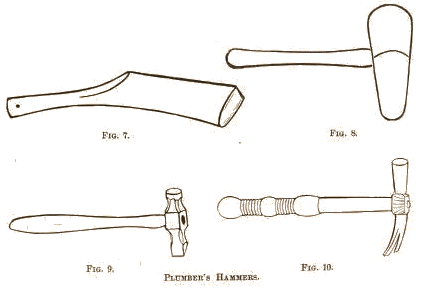
\includegraphics[width=1.0\textwidth]{popularsciencemo09newy_0033.png}
      \end{figure}
      \end{column}
  \end{columns}
\end{frame}

\begin{frame}{УДОБСТВО ИСПОЛЬЗОВАНИЯ.}
  \begin{columns}
    \begin{column}{0.6\textwidth}
      \raisebox{-.30em}{\Large\HandRight}\hspace{.25em} Инструмент должен
      быть удобен для использования.

      \bigskip

      \begin{itemize}
      \item Необходим понятный интерфейс, упрощающий корректное
        использование инструмента.
        % Некорректное использование криптографии инструмента может
        % привести к иллюзии защищённости, что гораздо хуже, чем если бы
        % инструмент не был использован в принципе.
        % См. также "Принцип наименьшего удивления."
      \item В идеале, инструмент должен оказывать минимальное влияние на
        рабочий процесс пользователя.
      \end{itemize}
    \end{column}
    \begin{column}{0.4\textwidth}
      \begin{figure}[htb]
        \centering
        
\includegraphics[height=.8\textheight]{hammer-use-0}
      \end{figure}
      \end{column}
  \end{columns}

\end{frame}

\begin{frame}{ДОСТУПНОСТЬ.}
  \raisebox{-.30em}{\Large\HandRight}\hspace{.25em} Инструмент должен
  предъявлять разумные требования, иначе его никто не будет
  использовать.

  \bigskip

  \begin{itemize}
  \item Необходима интеграция с существующим рабочим окружением
    пользователя, а не наоборот.
  \end{itemize}

  \begin{figure}[htb]
    \centering
    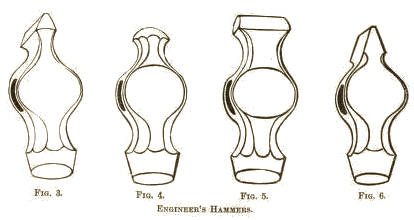
\includegraphics[height=.4\textheight]{hammer-01}
  \end{figure}
\end{frame}

\begin{frame}{ЭФФЕКТИВНОСТЬ.}
  \raisebox{-.30em}{\Large\HandRight}\hspace{.25em} Инструмент должен
  обеспечивать характеристики, которые были "по гарантии".\newline\newline

  \bigskip

  \begin{columns}
    \begin{column}{0.6\textwidth}
      \begin{itemize}
      \item Сообщество должно иметь возможность провести независимый аудит
        инструмента.
      \item Следовательно, исходный код инструмента, документация и
        описание протоколов должны быть доступны сообществу (желательно,
        под свободной лицензией.)
      \end{itemize}
    \end{column}
    \begin{column}{0.4\textwidth}
      \begin{figure}[]
        \centering
        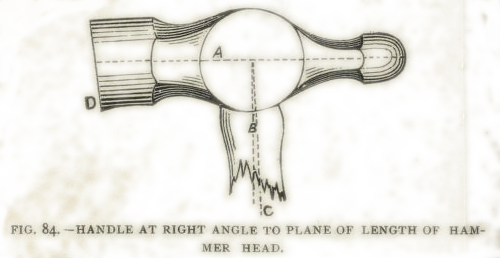
\includegraphics[width=1.1\textwidth]{hammer-00}
      \end{figure}
    \end{column}
  \end{columns}
\end{frame}

\begin{frame}{НАДЁЖНОСТЬ.}
  \raisebox{-.30em}{\Large\HandRight}\hspace{.25em} Если ``что-то
  пошло не так'', то инструмент должен сделать всё возможное, чтобы
  уменьшить урон.

  \bigskip

  \begin{quote}
    ``[...] a general principle of robustness: be conservative in what
    you do, be liberal in what you accept from others.'' -- Jon Postel
  \end{quote}

  \bigskip

  (Общий принцип надёжности Джона Постела: будьте консервативны в том,
  что делаете, и либеральны в том, что получаете от других.)

  \centering
  \pgfornament[width=0.5\textwidth]{88}

\end{frame}


%%%

\section{ДОСТУПНЫЕ ИНСТРУМЕНТЫ.}

\begin{frame}{ДОСТУПНЫЕ ИНСТРУМЕНТЫ.}
  \begin{itemize}
  \item GNU Privacy Guard (GnuPG)
  \item Off-The-Record Messaging (OTR)
  \end{itemize}
\end{frame}


%%%

\section{GNU PRIVACY GUARD.}

\begin{frame}{GNU PRIVACY GUARD.}
  \raisebox{-.30em}{\Large\HandRight}\hspace{.25em} GNU Privacy Guard
  (GnuPG) -- свободная программа шифрования информации и создания
  электронных цифровых подписей (ЭЦП).

  \vspace{5 mm}

  Задачи, решаемые с помощью GnuPG:
  \begin{itemize}
  \item Шифрование данных
  \item Электронная подпись данных
  \end{itemize}
\end{frame}


%%%

\subsection{СПАСИБО ЗА ВНИМАНИЕ.}

\begin{frame}{Спасибо за внимание!}
  \large

  Эл. почта: \url{poptsov.artyom@gmail.com}

  \medskip

  Презентация и её ``исходники'' под лицензией Creative Commons:
  \url{github.com/artyom-poptsov/talks/tree/master/defcon-nn/} \\[10pt]

  Спасибо, что выслушали  :-) \\[30pt]

  \bigskip

  \huge Вопросы?
\end{frame}

\begin{frame}{Лицензия}
  Copyright \textcopyright 2017 Artyom V. Poptsov
  <poptsov.artyom@gmail.com> \newline

  Права на копирование других изображений, использованных в данной
  работе, принадлежат их владельцам. \newline

  Данная работа распространяется на условиях лицензии Creative Commons
  Attribution-ShareAlike 4.0 International:
  \url{https://creativecommons.org/licenses/by-sa/4.0/}
\end{frame}


%%%

\end{document}

%%% 0x01.tex ends here
